\documentclass{homework}

\title{Project: Band Reject Filter}
\author{Kevin Evans}
\studentid{11571810}
\date{April 24, 2020}
\setclass{EE}{321}
\usepackage{amssymb}
\usepackage{mathtools}

\usepackage{amsthm}
\usepackage{amsmath}
\usepackage{slashed}
\usepackage{relsize}
\usepackage{threeparttable}
\usepackage{float}
\usepackage{booktabs}
\usepackage{boldline}
\usepackage{changepage}
\usepackage{physics}
\usepackage[inter-unit-product =\cdot]{siunitx}
\usepackage{setspace}

\usepackage[makeroom]{cancel}
\usepackage{pgfplots}

\usepackage{multicol}
\usepackage{tcolorbox}
\usepackage{enumitem}
\usepackage{times}
\usepackage{mhchem}
\usepackage{graphicx} 
\DeclareSIUnit{\year}{yr}
\usepackage[export]{adjustbox}
\usepackage{listings}
\usepackage{courier}
\renewcommand{\lstlistingname}{Code Snippet}
\usepackage{caption,subcaption} %multiline captions; subfigures

\lstset{basicstyle=\footnotesize\ttfamily,breaklines=true}
%\lstset{framextopmargin=50pt,frame=bottomline}
\lstset{language=Matlab,%
	%basicstyle=\color{red},
	breaklines=true,%
	morekeywords={matlab2tikz},
	keywordstyle=\color{blue},%
	morekeywords=[2]{1}, keywordstyle=[2]{\color{black}},
	identifierstyle=\color{black},%
	stringstyle=\color{mylilas},
	commentstyle=\color{mygreen},%
	showstringspaces=false,%without this there will be a symbol in the places where there is a space
%	numbers=left,%
%	numberstyle={\tiny \color{black}},% size of the numbers
%	numbersep=9pt, % this defines how far the numbers are from the text
	emph=[1]{for,end,break},emphstyle=[1]\color{red}, %some words to emphasise
	emph=[2]{zpkdata, tf}, emphstyle=[2]{\color{blue}},    
}

\usepackage{color} %red, green, blue, yellow, cyan, magenta, black, white
\definecolor{mygreen}{RGB}{28,172,0} % color values Red, Green, Blue
\definecolor{mylilas}{RGB}{170,55,241}

\renewcommand{\thesection}{\Roman{section}} 
\renewcommand{\thesubsection}{\arabic{section}.\arabic{subsection}}
\newcommand{\M}[1]{\mathrm{\mathbf{#1}}}
\begin{document}
	\maketitle
	\section{State model derivation}
	From the circuit, we can relate the currents at the node $v_o$ using KCL, \begin{align}
		\frac{v_o}{R_L} + i_2 & = \frac{v_i - v_o}{R_1} + i_1 \notag \\
		\left(\frac{1}{R_L} + \frac{1}{R_1}\right) v_o & = \frac{v_i}{R_1} + i_1 - i_2 \notag \\
		v_o & = \frac{R_L R_1}{R_L + R_1} \left(\frac{v_i}{R_1} + i_1 - i_2\right) \label{eq:vo1}
\intertext{Next, we can relate the relative voltages with KVL,}
		v_o & = v_c + v_2 \notag \\
			& = v_c + L_2 \dv{i_2}{t} \label{eq:vo2} \\
		v_o	& = v_i - v_1 \notag \\
			& = v_i - L_1 \dv{i_1}{t} \label{eq:vo3}
	\end{align}
	Combining the equations \eqref{eq:vo1} with \eqref{eq:vo2} and \eqref{eq:vo3}, then solving for the differential results in \begin{align}
		\dv{i_1}{t} & = \frac{1}{L_1} \left[ \left(1 - \frac{R_L}{R_L + R_1}\right) v_i - \frac{R_L R_1}{R_L + R_1} i_1 + \frac{R_L R_1}{R_L + R_1} i_2  \right] \\
		\dv{i_2}{t} & = \frac{1}{L_2} \left( \frac{R_L}{R_L + R_1} v_i + \frac{R_L R_1}{R_L + R_1} i_1 - \frac{R_L R_1}{R_L + R_1} i_2 - v_c\right)
		\shortintertext{Lastly, we can equate the second inductor current $i_2$ with the capacitor current,}
		\dv{v_c}{t} & = \frac{1}{C} i_2
	\end{align} 
	At this point, the differentials from the inductors and capacitors have been related and can be assembled into a state matrix, where the state matrix represents the inductor currents $i_1$ and $i_2$, as well as the capacitor voltage $v_c$ through time. The elements of the differential matrix $\M{\dot{X}}$ is then equated to eq. ($4$), ($5$), and ($6$), resulting in \begin{align*}
		\M{\dot{X}} & = \M{A} \M{X} + \M{B} \M{G} \\
		\left[\begin{matrix}
			\dv{i_1}{t} \\
			\dv{i_2}{t} \\
			\dv{v_c}{t}
		\end{matrix} \right] &
		=
		\left[ \begin{matrix}
			-\frac{1}{L_1} \left( \frac{R_L R_1}{R_L + R_1} \right) & \frac{1}{L_1} \left( \frac{R_L R_1}{R_L + R_1} \right) & 0 \\
			\frac{1}{L_2} \left( \frac{R_L R_1}{R_L + R_1} \right) & -\frac{1}{L_2} \left( \frac{R_L R_1}{R_L + R_1} \right) & - \frac{1}{L_2} \\
			0 & 1 / C & 0
		\end{matrix} \right]
		\left[
			\begin{matrix}
				i_1 \\
				i_2 \\
				v_c
			\end{matrix}
		\right]
		+
		\left[ \begin{matrix}
			\frac{1}{L_1} \left( 1 - \frac{R_L}{R_L + R_1}\right) \\
			\frac{1}{L_2} \left( \frac{R_L}{R_L + R_1}\right) \\
			0 \end{matrix}
		\right] v_i(t)
		\intertext{	The output matrix has a singular element of $v_o$, which is trivially found through the currents passing through the load resistor, effectively by rearranging \eqref{eq:vo1}.}
		\M{Y} & = \M{C} \M{X} + \M{D} \M{G} \\
		\left[v_o\right] &
		=
		\left[ \begin{matrix}
			\frac{R_L R_1}{R_L + R_1} & -\frac{R_L R_1}{R_L + R_1} & 0
		\end{matrix}\right] \M{X} + \left[
	\frac{R_L}{R_L + R_1}\right] v_i(t)
	\end{align*}
	\subsection*{MATLAB numeric estimations}
	Using MATLAB, we can use the control systems toolbox to find the transfer function of this state matrix numerically. If we input the matrices into variables, the \texttt{ss} and \texttt{tf} commands may be used to numerically determine the transfer function $H(s)$.  The resulting plots are shown below in Figure \ref{fig:ssbode} and \ref{fig:ssresp}, using the code from Snippet \ref{lst:mtx}.	
	
	\begin{figure}[H]
		\centering
		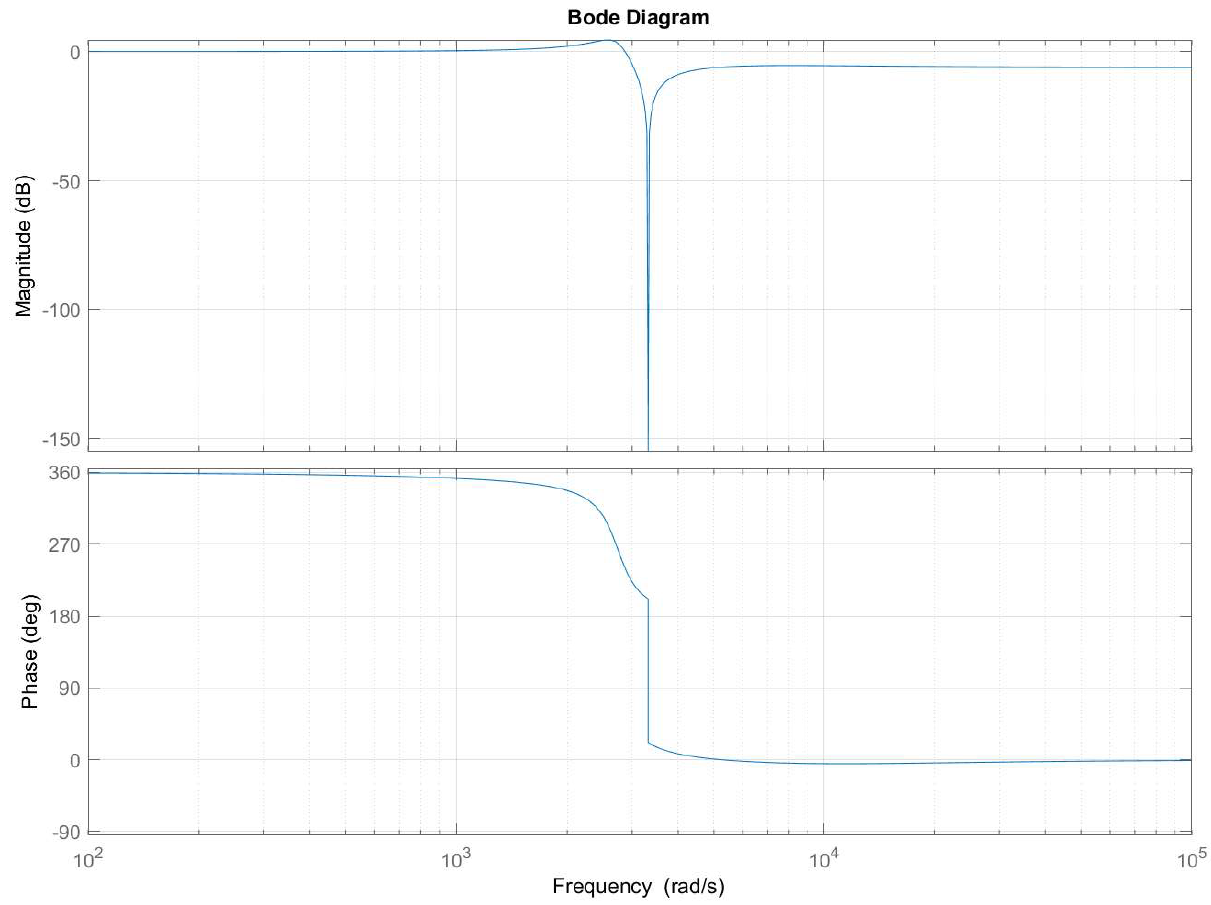
\includegraphics[width=0.7\linewidth]{ssbode}
		\caption{Bode diagram of the transfer function calculated using the state space matrices.}
		\label{fig:ssbode}
	\end{figure}
	
	\begin{figure}[H]
		\centering
		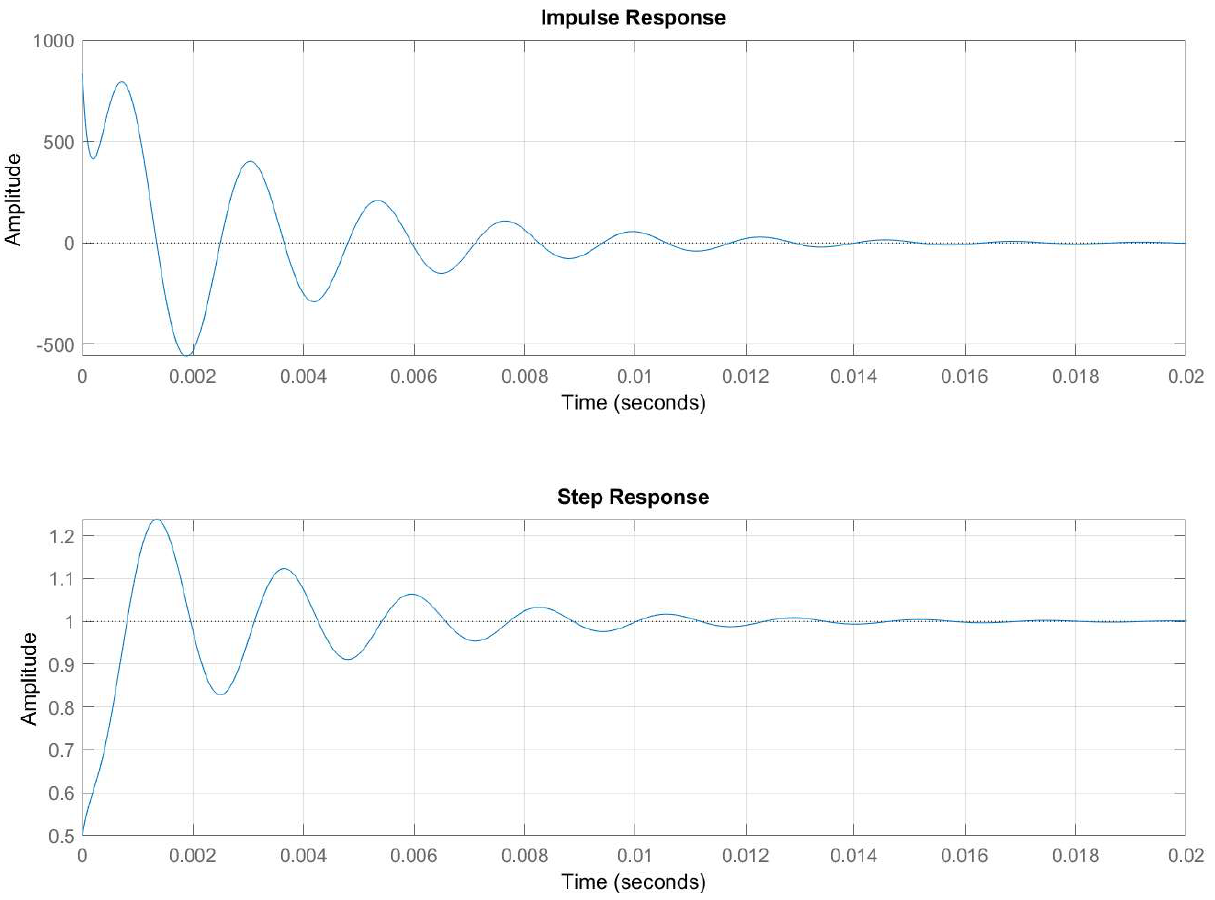
\includegraphics[width=0.7\linewidth]{ssresp}
		\caption{Time domain responses of the transfer function calculated using the state space matrices.}
		\label{fig:ssresp}
	\end{figure}

	\begin{figure}[H]
	\begin{lstlisting}[language=matlab, caption={MATLAB code for solving for the transfer function using state space equations.},label={lst:mtx}]
A = [ -4166.67,   4166.67,    0;
       2500.00,  -2500.00, -100;
          0.00, 109890.10,    0];  
B = [83.33;
     50.00;
      0.00];
C = [25, -25, 0];
D = [0.5];

% solve system and system->tf
system = ss(A, B, C, D);
H      = tf(system);

% plot a bode plot
bode(H);

% plot: impulse, step, and bode plots
%subplot(2, 1, 1);
figure;
impulse(H);
grid on;

%subplot(2, 1, 2);
figure;
step(H);
grid on;

%subplot(4, 1, [3, 4]);
figure;
bode(H);
grid on;
	\end{lstlisting}
\end{figure}	
	\pagebreak
	\section{Impulse and step response}
	We can convert the circuit to the $s$-domain and use a simple voltage divider to find the transfer function $H(s)$. First, the components are converted to their $s$-domain equivalent, as shown in Figure \ref{fig:poop}(a). Next, the circuit is reduced, allowing us to use a simple voltage divider to calculate the transfer function. This is shown in Figure \ref{fig:poop}(b). The impedances can be calculated as \begin{align*}
		Z_A & = \left(R_1 \parallel s L_1\right) = \left[50 \parallel s \left(\num{6e-3}\right)\right] \\
			& = \frac{ 150 s}{25000 + 3 s} \\
		Z_B & = \left[R_L \parallel \left(Z_{L2} + Z_C\right)\right] \\
			& = 50 \parallel \left[s \left(\num{10e-3}\right) + \frac{1}{s \left(\num{9.1e-6}\right)} \right] \\
			& = \frac{ 50 \left(s^2 + \num{1.0989e7}\right) }{ s^2 + 5000 s + \num{1.0989e7}}
	\end{align*}
	From the voltage divider technique, the $s$-domain transfer function is found as \begin{align}
		H(s) & = \frac{Z_B}{Z_A + Z_B} \notag \\
			& = \frac{ 0.5 s^3 + 4166.67 s^2 + 5494500 s + \num{4.57875e10} }{s^3 + 6666.67 s^2 + 10989000 s + \num{4.57875e10}} \label{eq:H}
	\end{align}

	\begin{figure}[h]
		\begin{subfigure}{0.68\linewidth}
			\centering
			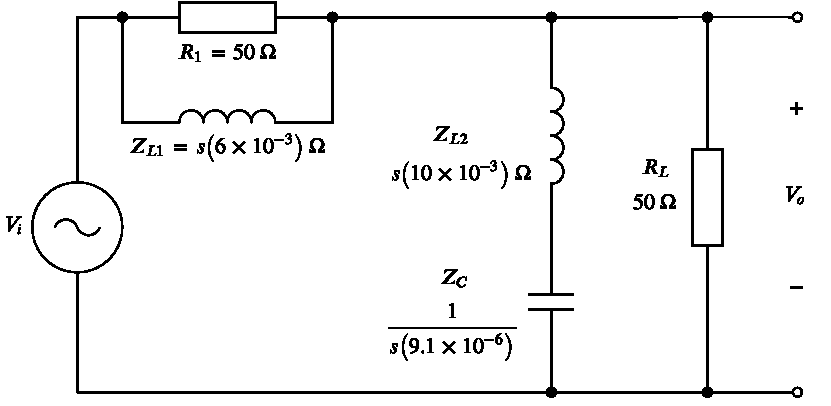
\includegraphics[width=\linewidth]{projpre.pdf}
			\caption{}
		\end{subfigure}
		\begin{subfigure}{0.3\linewidth}
			\centering
			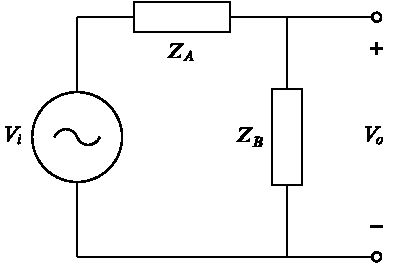
\includegraphics[width=\linewidth]{proj.pdf}
			\caption{}
		\end{subfigure}
		\caption{Circuit diagrams of the filter (a) in the $s$-domain and (b) reduced to two impedances.}
		\label{fig:poop}
	\end{figure}
	
	\pagebreak
	\subsubsection*{Factoring using MATLAB}
	This transfer function was entered into a MATLAB script to determine the zero and pole locations, as well as the residues. Using the \texttt{zpkdata} and \texttt{residue} functions, the transfer function was factored using \lstlistingname \space \ref{lst:factor} as
	\begin{align*}
		H(s) & = 0.5 + \frac{1307.4886}{s + 6096.1298}
			- \frac{237.0768-j418.2}{s + 285.2701-j2725.7171}
			- \frac{237.0768+j418.2}{s + 285.2701+j2725.7171}
	\end{align*}
	\noindent From the MATLAB code, the poles and zeros are found to be:
	
	\vspace{1em}
	\noindent
	\begin{tabular}{ll}
		$\bullet$ Poles: & $s_{p1} = -6.0961$ \\
		& $s_{p2} = -0.2853 + j2.7257$ \\
		& $s_{p3} = s_{p2}^* = -0.2853 - j2.7257$ \\
		& \\
		$\bullet$ Zeros: & $s_{z1} = -8333.33$ \\
		& $s_{z2} = j3315$ \\
		& $s_{z3} = s_{z2}^* = -j3315$
	\end{tabular}
	
	\vspace{1em}
	
	\begin{figure}[H]
	\begin{lstlisting}[language=matlab, caption={MATLAB code for factoring the transfer function.},label={lst:factor}]
% coefficients of the transfer function:
% order:
% s^   3,       2,        1,          0
N = [0.5, 4166.67,  5494500, 4.57875e10]; % numerator
D = [  1, 6666.67, 10989000, 4.57875e10]; % denominator

% generate transfer function, H(s)
H            = tf(N, D);
[z, p,    k] = zpkdata(H, 'v');  % zeros, poles, gain
[r, ptmp, k] = residue(N, D);    % residues r -> are the K_i values

% print out the residues over the poles
for i = 1 : 3
	fprintf("\n%d -> %s\n\t----------------------\n\t%s\n", ...
		i, num2str(r(i)), num2str(p(i)) );
end
	\end{lstlisting}
	\end{figure}

	\pagebreak
	\subsection{Impulse Response}
	If we transform the unit impulse function $\delta(t)$ to the $s$-domain, we can multiply it by the transfer function to determine the response of the circuit. As the impulse function simply is $1$ in the $s$-domain, \begin{align*}
		Y_\delta(s) & = H(s) X(s) \\
			& = 0.5 + \frac{1307.4886}{s + 6096.1298}
			- \frac{237.0768-j418.2}{s + 285.2701-j2725.7171}
			- \frac{237.0768+j418.2}{s + 285.2701+j2725.7171}
		\end{align*}
	We can take the inverse Laplace transform to get the response in the time domain. The first term, $0.5$, becomes the coefficient to another impulse function and is negligible. For the last two terms, which have conjugates in both the denominator and numerator, we can use Table $12.3$ from Nilsson/Riedel (p. 469) to transform the terms into a cosine function,
	\begin{align*}
		\mathcal{L}^{-1} \left\{ Y_{\delta(s)} \right\} & = 1307.4886 e^{-6096.1298t}
			- 2 \abs{237.0768 + j 418.2} e^{-285.2701 t} \cos(2725.7171 t + \tan(\frac{418.2}{2725.7171})) \\
			y_\delta (t)	& = 1307.4886e^{-6096.1298t} - 961.45 e^{-285.2701t} \cos(2725.7171t + 60.45^\circ)
	\end{align*}
	As shown in Figure \ref{fig:part21impulse} below, plotting this function using MATLAB, we can see that the impulse response is identical to the response from Part I. The code used to plot this is shown in the Snippet \ref{lst:impulseplot} below.
	\begin{figure}[H]
		\centering
		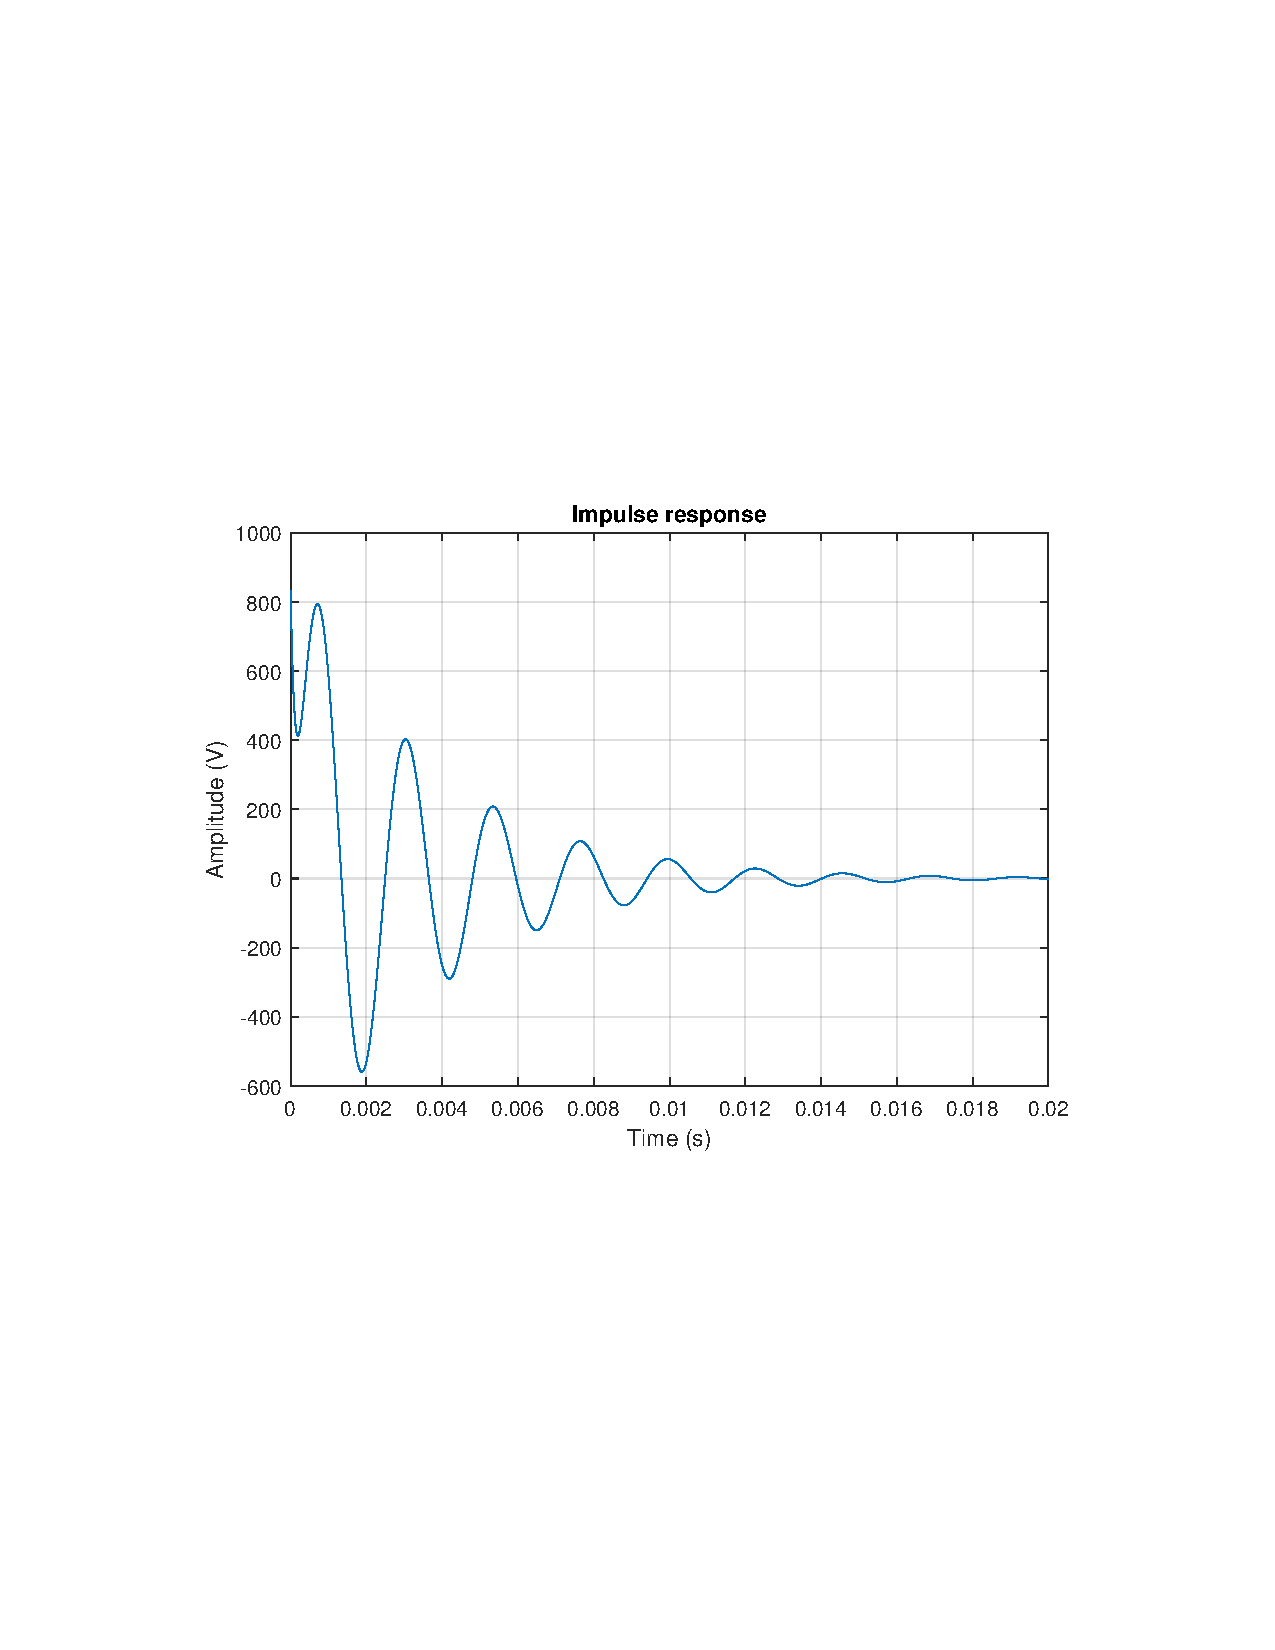
\includegraphics[width=0.65\linewidth,clip,trim=4cm 8.5cm 3cm 8.5cm]{part2_1impulse}
		\caption{Plot of the impulse response in the time domain.}
		\label{fig:part21impulse}
	\end{figure}
	\vspace{-2em}
	\begin{figure}[H]
		\begin{lstlisting}[language=matlab, caption={MATLAB code for plotting the impulse response.},label={lst:impulseplot}]
dt = 5e-6;
t  = (0:dt:20e-3);
y  = 1307.4886 .* exp(-6096.13 .* t) ...
     - 2 .* 480.725 .* exp(-285.2701.*t) .* cos(2725.7171.*t + deg2rad(60.45));

figure;
plot(t, y);
title('Impulse response');
xlabel('Time (s)');
ylabel('Amplitude (V)');
grid on;
		\end{lstlisting}		
	\end{figure}
	\pagebreak
	\subsection{Step Response}
	Next, the step response can be calculated using the transfer function found earlier. Starting from \eqref{eq:H}, we can find the step response first in the $s$-domain, \begin{align*}
		Y(s) & = X(s) H(s) \\
			& = \frac{1}{s} H(s) \\
			& = \frac{ 0.5 s^3 + 4166.67 s^2 + 5494500 s + \num{4.57875e10} }{s^4 + 6666.67 s^3 + 10989000 s^2 + \num{4.57875e10}s}
	\end{align*}
	The output function $Y(s)$ remained the same, but with only the order of the denominator incremented. The transfer function was factored using the same MATLAB code as the impulse function, Snippet \ref{lst:factor}, and was shown to be \begin{align*}
		Y(s) & =  \frac{1}{s} - \frac{0.2145}{s + 6096.1298}
			- \frac{0.1428 - j0.1019}{s + 285.2701 + j2725.7171}
			- \frac{0.1428 + j0.1019}{s + 285.2701 - j2725.7171}
	\end{align*}
	If we take the inverse Laplace transform, we can find the output in the time domain $y(t)$. This uses the same transformation pairs listed in Table 12.3 of Nilsson/Riedel. 
	\begin{align*}
		y(t) & = \mathcal{L}^{-1} \left\{ Y(s) \right\} \\
			& = 1.0 - 0.2145 e^{-6096.1 t} + 0.350858 e^{-285.3 t} \cos(2725.7 t + 144.489^\circ)
	\end{align*}
	If we plot the response in the time domain using MATLAB, we can see that this is equivalent to the plots from Part I. This plot is shown in Figure \ref{fig:part22step} using the code from Snippet \ref{lst:stepplot}.
	\begin{figure}[H]
		\centering
		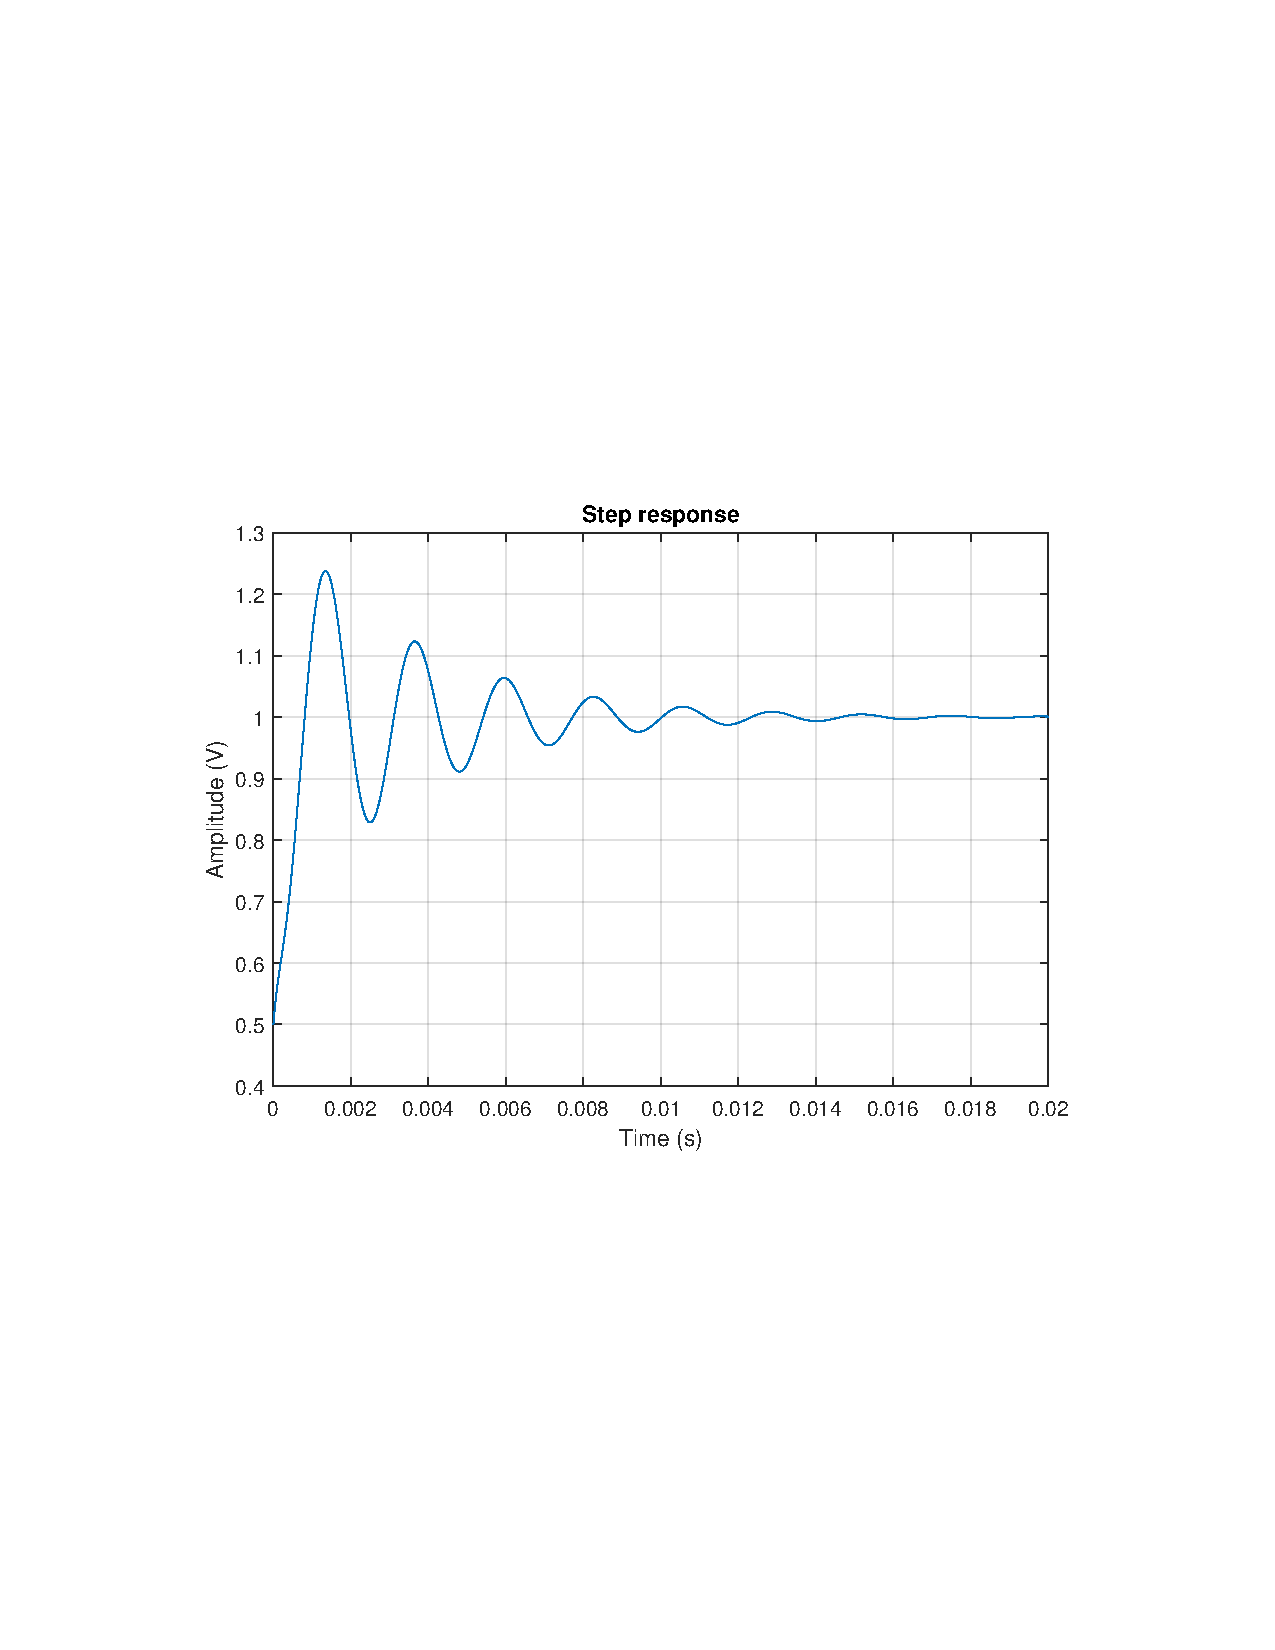
\includegraphics[width=0.7\linewidth,clip,trim=4cm 8.5cm 3cm 8.5cm]{part2_2step}
		\caption{Plot of the step response in the time domain.}
		\label{fig:part22step}
	\end{figure}
	\begin{figure}[H]
		\begin{lstlisting}[language=matlab, caption={MATLAB code for plotting the step response.},label={lst:stepplot}]
dt = 5e-6;
t  = (0:dt:20e-3);
y = 1.0 + -0.2145 .* exp(-6.0961e3 .* t) ...
    + 2 .* 0.175429 .* exp(-0.2853e3 .* t) .* cos(2.7257e3 .* t + deg2rad(144.489));
figure;
plot(t, y);
title('Step response');
xlabel('Time (s)');
ylabel('Amplitude (V)');
grid on;
		\end{lstlisting}
	\end{figure}

	\subsection{Frequency response}
	From the original transfer function calculation, eq. \eqref{eq:H}, we can use the \texttt{bode} function in MATLAB to plot this frequency response of the circuit. This was accomplished by appending \texttt{bode(H);} to the MATLAB code in Snippet \ref{lst:factor}, resulting in the plot shown in Figure \ref{fig:part23bode}.
	
	\begin{figure}[H]
		\centering
		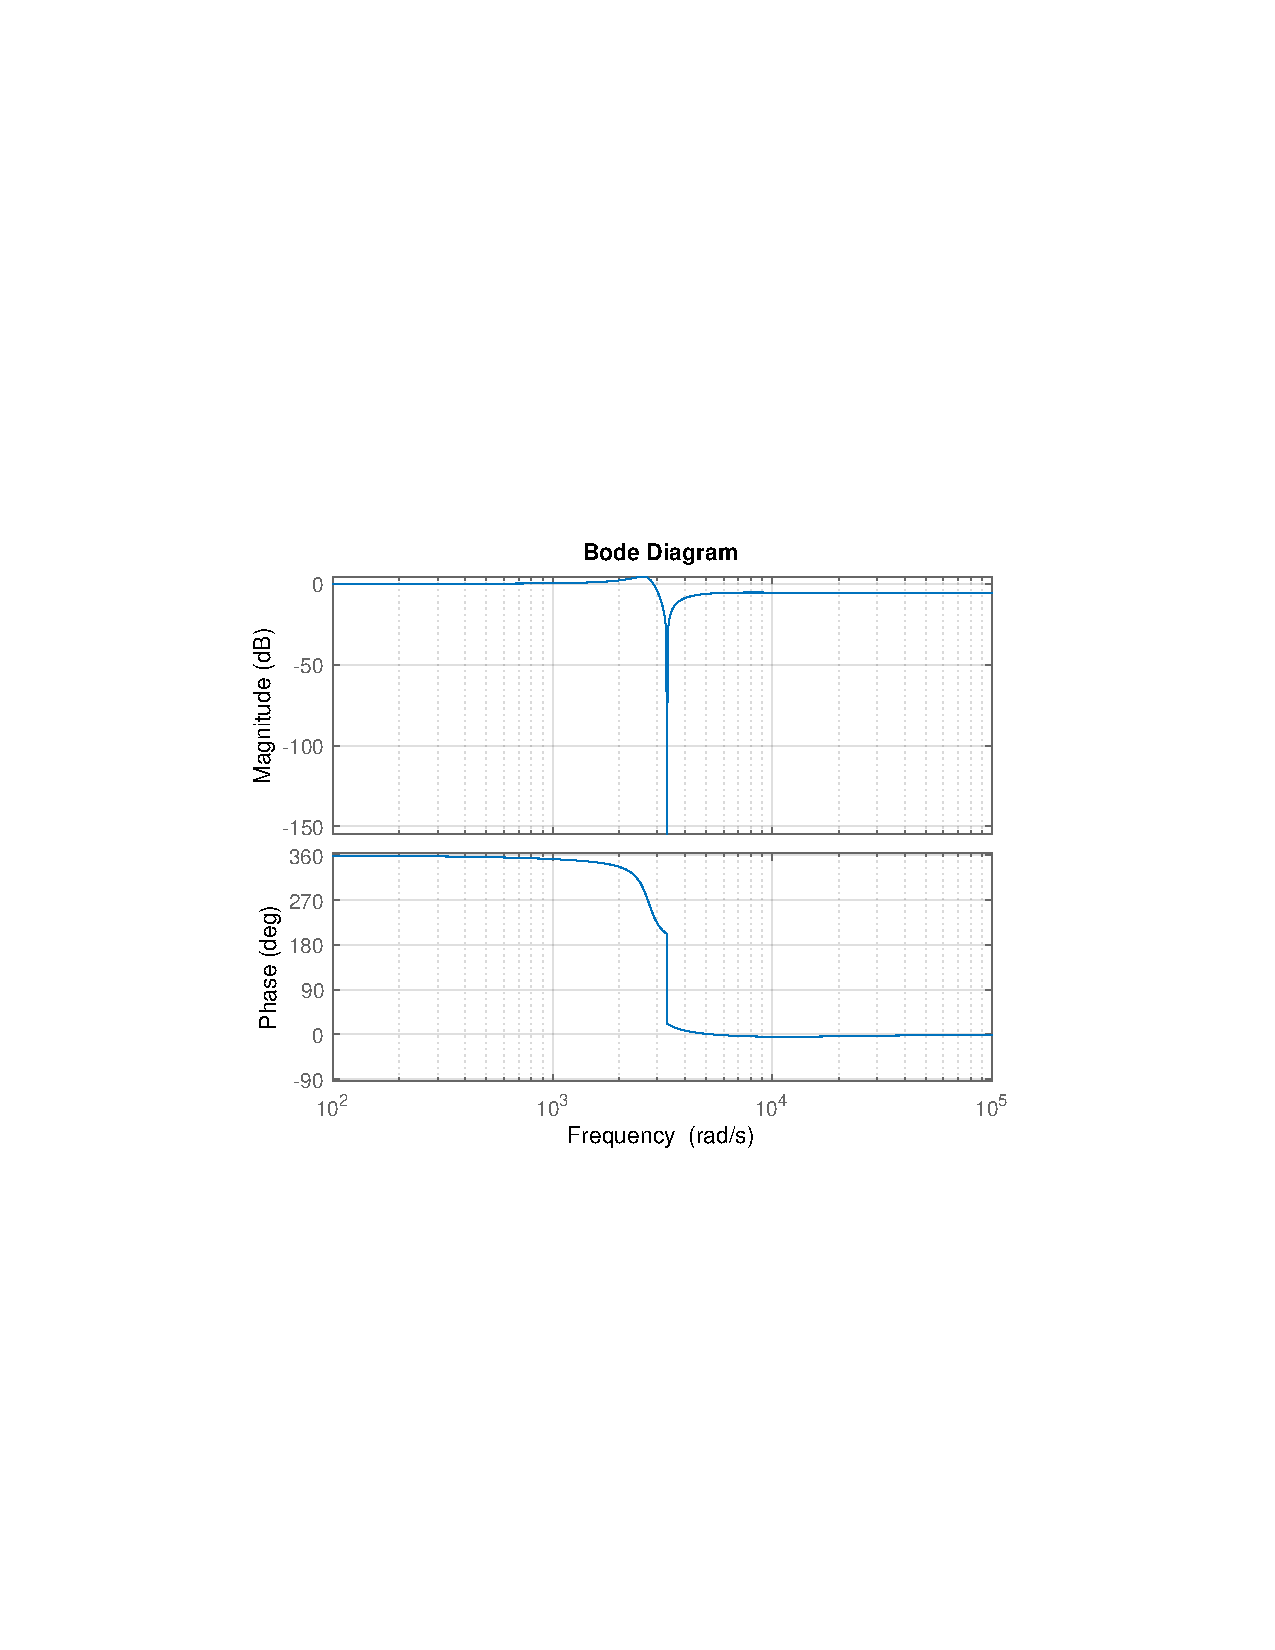
\includegraphics[width=0.7\linewidth,clip,trim=4cm 8.5cm 3cm 8.5cm]{part2_3bode}
		\caption{Plot of the step response in the time domain.}
		\label{fig:part23bode}
	\end{figure}

	\pagebreak
	\section{Differential expression}
	From Part I, it is clear that using the output matrix $\M{Y}$ containing $v_o$, \begin{align*}
		v_o & = \frac{R_1 R_L}{R_1 + R_L} \left( i_1 - i_2 \right) + \frac{R_L}{R_1 + R_L} v_i \\
		\intertext{Where $v_o$, $i_1$, $i_2$, and $v_i$ are all functions of $t$. If we take the third derivative of both sides, }
		\dddot{v_o} & = \frac{R_1 R_L}{R_1 + R_L} \left( \dddot{i_1} - \dddot{i_2} \right) + \frac{R_L}{R_1 + R_L} \dddot{v_i} \tag{*}
		\intertext{If we related the inductor currents to the input and output voltages,}
		v_o & = v_i - L_1 \dot{i_1} \\
		\frac{v_o}{R_L} + i_2 & = \frac{v_i - v_o}{R_1} + i_1
		\intertext{Continually differentiating these and rearranging results in}
		\dddot{i_1} & = \frac{\ddot{v_i}}{L_1} - \frac{\ddot{v_o}}{L_1} \\
		\dddot{i_2} & = \frac{1}{L_2} \left(\ddot{v_o} - \frac{1}{C} \dot{i_2} \right) \\
			& = \frac{ \ddot{v_o} }{L_2} - \frac{1}{L_2 C} \left[
				\frac{1}{R_1} \dot{v_i}
				-\left(\frac{1}{R_1} + \frac{1}{R_L} \right) \dot{v_o}
				 + \frac{v_i}{L_1}
				 - \frac{v_o}{L_1}
			 \right]
	\end{align*}
	If we now substitute $\dddot{i_1}$ and $\dddot{i_2}$ into (*) and rearrange terms,
	\begin{align*}
		\dddot{v_o} + \frac{R_1 R_L}{R_1 + R_L}	 \left[
			\left(\frac{1}{L_1} + \frac{1}{L_2}\right) \ddot{v_o}
			+ \frac{1}{L_2 C} \left( \frac{1}{R_1} + \frac{1}{R_L}\right) \dot{v_o}
			+ \frac{1}{L_2 C L_1} v_o
		\right] \\
		= \frac{R_1 R_L}{R_1 + R_L} \left[
			\frac{1}{L_1} \ddot{v_i}
			+ \frac{1}{L_2 C R_1} \dot{v_i} 
			+ \frac{1}{L_2 C L_1} v_i
		\right] + \frac{R_L}{R_1 + R_L} \dddot{v_i}
	\end{align*}
	Simplifying it some more, it matches the given differential equation, \begin{align*}
		\dddot{v_o} + \frac{R_1 R_L}{R_1 + R_L} \left(\frac{1}{L_1} + \frac{1}{L_2}\right) \ddot{v_o} + \frac{1}{L_2 C} \dot{v_o} + \frac{R_1 R_L}{R_1 + R_L} \frac{1}{L_1 L_2 C} v_o \\
		= \frac{R_L}{R_1 + R_L} \left[
			\dddot{v_i}
			+ \frac{R_1}{L_1} \ddot{v_i}
			+ \frac{1}{L_2 C} \dot{v_i}
			+ \frac{R_1}{L_1 L_2 C} v_i
		\right] \qed
	\end{align*}
	\pagebreak
	\section{Numeric convolution}
	Using MATLAB, we can estimate the convolution using the \texttt{conv} function over discrete times. The numeric convolution results in plots that are nearly identical to the plots found earlier. Shown in Figures \ref{fig:part4step} and \ref{fig:part4impulse} are the step and impulse responses found using the numeric convolution. The MATLAB code used to generate these plots is listed in Snippet \ref{lst:conv}.
	
	\begin{figure}[H]
		\centering
		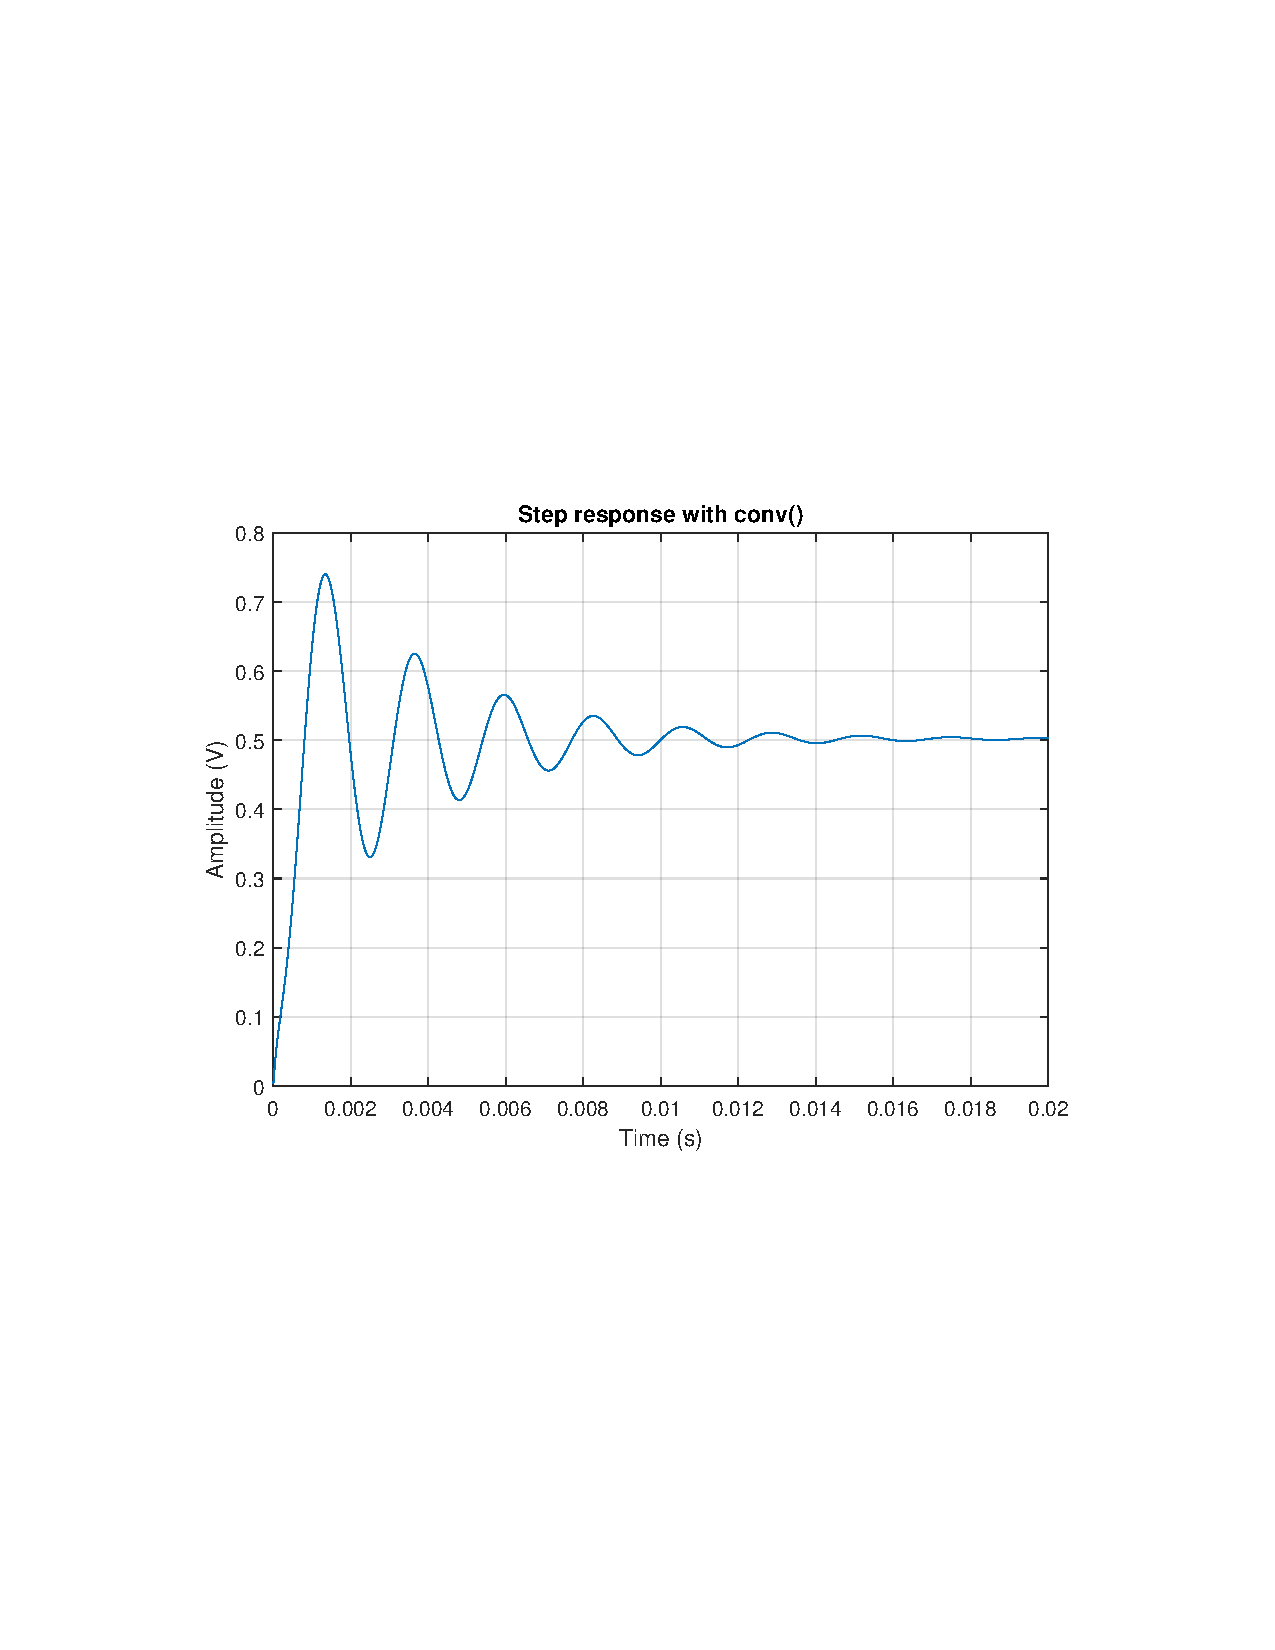
\includegraphics[width=0.7\linewidth,clip,trim=4cm 8.5cm 3cm 8.5cm]{part4_step}
		\caption{Step response of the transfer function using MATLAB's \texttt{conv} command.}
		\label{fig:part4step}
	\end{figure}
	\vspace{-1em}
	\begin{figure}[H]
		\centering
		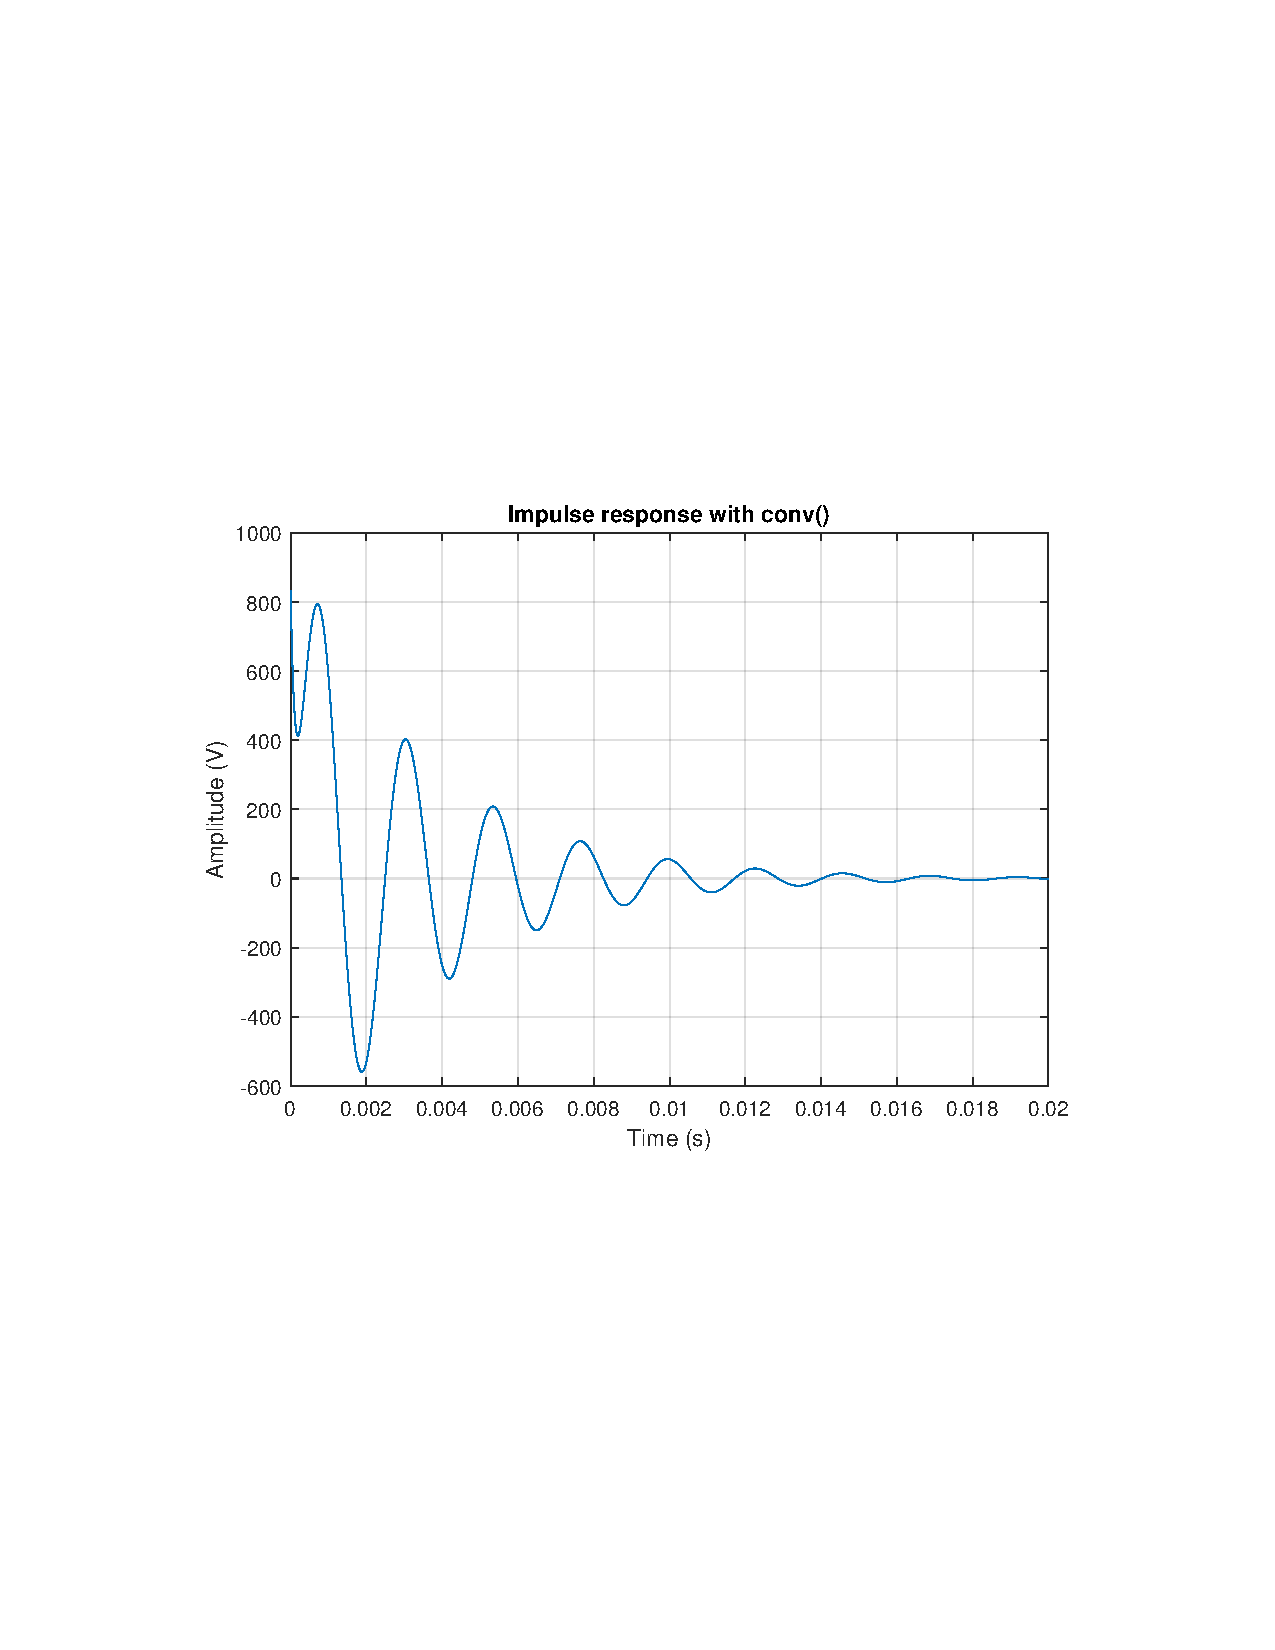
\includegraphics[width=0.7\linewidth,clip,trim=4cm 8.5cm 3cm 8.5cm]{part4_impulse}
		\caption{Impulse response of the transfer function using MATLAB's \texttt{conv} command.}
		\label{fig:part4impulse}
	\end{figure}

	\begin{figure}[H]
	\begin{lstlisting}[language=matlab, caption={MATLAB code for the convolutions.},label={lst:conv}]
% reusing the transfer function from Part II.
dt = 5e-6;
t  = (0:dt:20e-3);
h  = 1307.4886 .* exp(-6096.13 .* t) ...
     - 2 .* 480.725 .* exp(-285.2701.*t) .* cos(2725.7171.*t + deg2rad(60.45));

% input functions:
u  = ones(1, 2 * length(t));       % unit step, filled with 1
d  = [1/dt zeros(1, length(t)-1)]; % impulse, a spike then filled with 0

% numerically find the convolutions for both
s  = conv(h, u) * dt; % unit step
s2 = conv(h, d) * dt; % impulse

figure;
plot(t, s(1:length(t)));
title('Step response with conv()');
xlabel('Time (s)');
ylabel('Amplitude (V)');
grid on;

figure;
plot(t, s2(1:length(t)));
title('Impulse response with conv()');
xlabel('Time (s)');
ylabel('Amplitude (V)');
grid on;
	\end{lstlisting}
\end{figure}
\end{document}